In the December 2019 workshop\textit{ Implications of Artificial Intelligence for Cybersecurity}\cite{Evans_2008}, one of the key takeaways identified was the need to expand the connections between cyber security and applications of artificial intelligence and machine learning. In this work we have so far focused on making cyber security measurable, focusing on instrumentation for automation and autonomy. Programmatic access to security metrics through automation opens up a wide variety of applications involving, and can itself be improved by, current techniques in machine learning. In this section we describe the design details for the experiments we are developing using the SMaaS environment. While adversarial AI and attacks on ML models are areas of concern today, the direction of this work is \textit{not} in applying SMaaS to evaluate the security of machine learning. Instead, we propose to investigate the use of specific machine learning techniques to improve cyber security through the metrics framework we developed above. 

Machine learning techniques can be described by the 4 key types of of problems they solve. \textbf{Clustering} problems try to find groupings in data sets by minimizing distances from members of the same group and maximizing distances between members of differing groups. \textbf{Classification} problems map new instance data onto a discrete set of values representing categories or labels, while \textbf{regression} maps new data onto a continuous set of values. \textbf{Rule extraction}\cite{Denker} is a statistical 
inference method used to predict responses from given input patterns. 

It is also common to describe machine learning by one of four types of learning used. \textbf{Supervised} learning is provided labeled training data to build models from, while \textbf{unsupervised} learning is trained on unlabeled data. \textbf{Semi-supervised} learning is used with a mix of labeled and unlabeled data. \textbf{Reinforcement} learning\cite{Sutton_Barto_2018} maximizes values from an internal scoring functions to learn a model about the environment. 

Machine learning is a fast moving research area. We consult the 2019 \textit{Deep Learning in Mobile and Wireless Networking: A Survey}, \cite{Zhang_Patras_Haddadi_2019}, 2018 \textit{A comprehensive survey on machine
learning for networking}\cite{Boutaba_2018}, and the 2018 \textit{Machine Learning and Deep Learning Methods for Cybersecurity}\cite{Xin_Kong_Liu_Chen_Li_Zhu_Gao_Hou_Wang_2018} to identify current techniques and canonical literature for our topic. 

MulVal Facts : Datalog facts defining system model: (Hosts, Policies, Principals, Vulnerabilities, Interaction Rules) + (Attacker Location, Goal)
MulVal Output: DAG of possible paths attacker can reach goal (nxn connectivity matrix)

\section{Security Metric Prediction}

Problem Type: Classification and Regression problem.

There are quite a few scenarios that can be described as ‘Metric Prediction’. In general we approach these as supervised categorical classification or regression tasks, where SMaaS is used to create a labeled dataset of network models or attack graphs with the resulting security metric(s). Training and validation proceed as usual, with the resulting model able to predict the metric of new network states or topologies without needing the SMaaS system.

1a. Vulnerability Score Perturbation to predict metric


\begin{figure}[ht]
\centering
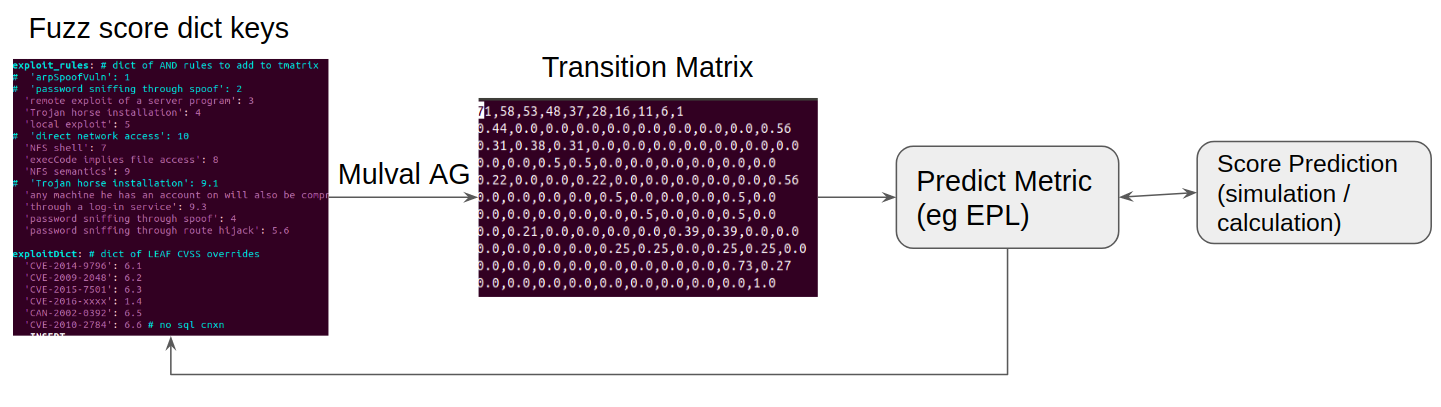
\includegraphics[width=.9\textwidth]{resource/img/ch_future/1a.png}
\caption{Learning Metrics from Vulnerability Score}
\label{fig:final:1a}
\end{figure} 

Goal: Given a weighted transition matrix $\longrightarrow$ predict specific metric

Method: Fuzz vulnerability weights (won't affect AG structure)
\begin{itemize}
\item Find best fit function (LR, …)
\item Compare time/perf over simulation for small/med/large matrixes
\item Compare performance for different metrics (within/outside same class)
\item Fuzz subset of vulns for PCA or confuse
\end{itemize}

1b. Vulnerability Placement Fuzzing 

\begin{figure}[ht]
\centering
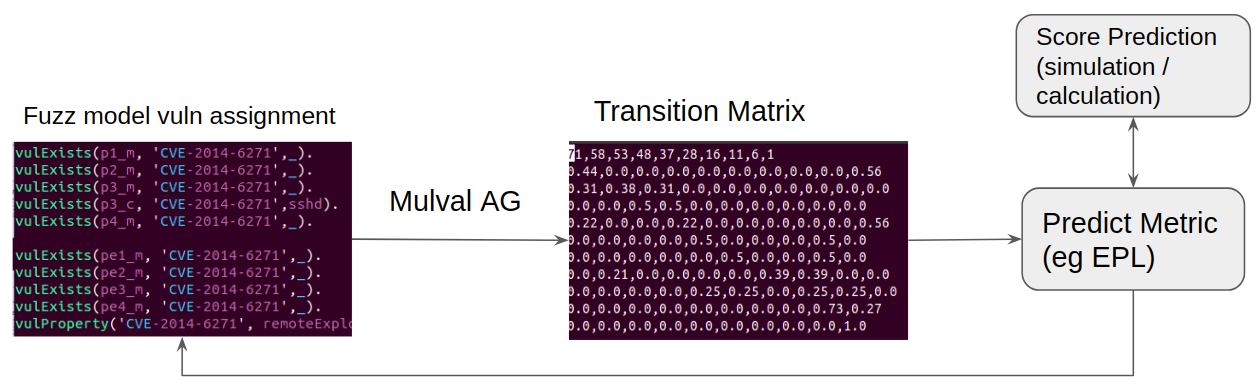
\includegraphics[width=.9\textwidth]{resource/img/ch_future/1b.png}
\caption{Learning Metrics from Vulnerability Placement}
\label{fig:final:1b}
\end{figure} 

Goal: Given a MulVal model $\longrightarrow$ predict specific metric

Method: Fuzz vulnerability placements (will affect AG structure)

\begin{itemize}
\item Can we learn if an AG will be produced (connectedness)?
\item Can we predict any metrics?
\item Might be a good application for GNNs 
\item Could either learn on tmatrix (easy) or MulVal model (harder)
\end{itemize}




1c. Network Model Fuzzing 


\begin{figure}[ht]
\centering
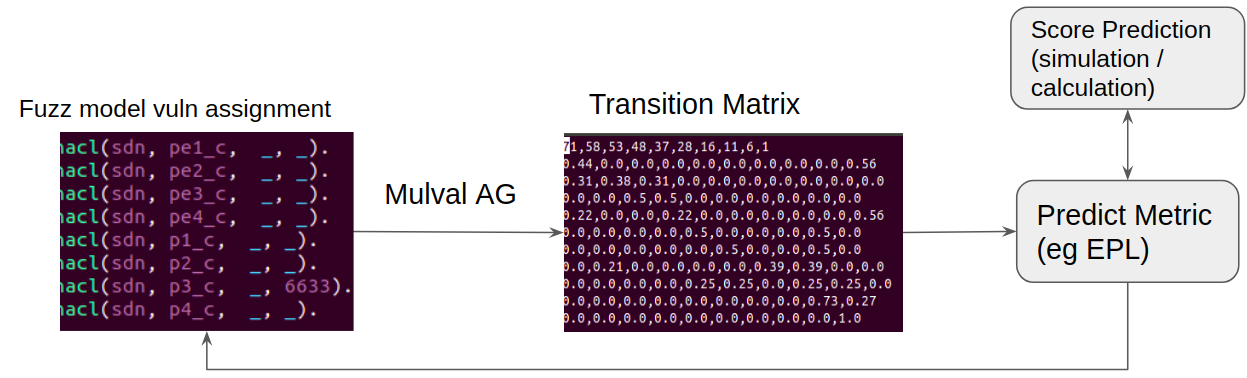
\includegraphics[width=.9\textwidth]{resource/img/ch_future/1c.png}
\caption{Learning Metrics from Network Topology}
\label{fig:final:1c}
\end{figure} 


Goal: Given a MulVal model $\longrightarrow$ predict specific metric

Method: Fuzz network facts (will affect AG structure)
\begin{itemize}
\item Can we learn if an AG will be produced (connectedness)?
\item Can we learn how to make a valid Network model?
\item Prolog syntax/token understanding needed
\end{itemize}


\section{Model Enhancements}

The reliability of a measurement depends on the reliability of the input. \textit{Garbage in, garbage out} is especially true for model based calculations. In Section \ref{sec:automation:infra} we discussed the role \textit{interaction rules} play in defining the possible attacks against a system, and that a model missing relevant interaction rules will falsely report no possible attacks when, in fact, they do exist. 

In order to ensure complete coverage of IRs for the domains we model, we need to have these rules defined systematically. A good starting point is MITRE's CAPEC\cite{Corporation}, the Common Attack Pattern Enumeration and Classification dataset. While this corpus includes primarily application type attacks, another dataset, CyBOX (recently moved into STIX), includes attack patterns observable at lower layers like infrastructure and physical such as those we defined in Section \ref{sec:automation:infra}.  
Recall from Section \ref{sec:background:modeling} that an interaction rule can be represented as a \textit{Horn Clause} of the form $A\xleftarrow[]{} B_1, B_2,\dots, B_n $, where $B_1, B_2,\dots, B_n $ are facts defining preconditions that must be true to assert $A$ is true. Both CAPEC and CyBOX include preconditions with each attack pattern, but sadly they chose to make this field free text and not categorical. Noel in \cite{Noel_2018} describes text mining techniques for many scenarios but prerequisite enumeration is not one of them. 

\begin{verbatim}
This attack requires the following:
1. The application uses environment variables.
2. An environment variable exposed to the user is vulnerable to a buffer overflow.
3. The vulnerable environment variable uses untrusted data.
4. Tainted data used in the environment variables is not properly validated. 
\end{verbatim}

The example above lists the CAPEC preconditions for the \textit{authentication abuse, ID:114} attack pattern. There are currently 517 unique attack patterns, along with associated prerequisites and \textit{consequences}, which capture post conditions like privileges gained from a successful attack. Our goal in this work is to expand the knowledge base for threat model generation to more accurately represent known patterns, and to accommodate future patterns as they become known.

\subsection{Interaction Rule Mining}


Problem Type: Association Rule Learning


\begin{figure}[ht]
\centering
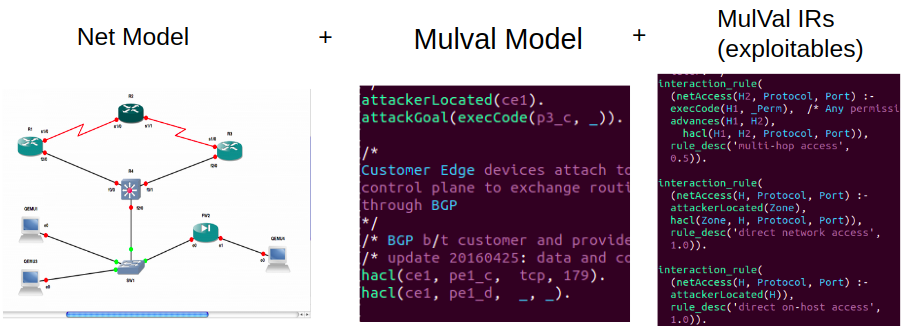
\includegraphics[width=.9\textwidth]{resource/img/ch_future/rule_learning.png}
\caption{Association Rule Learning}
\label{fig:final:learn_rule}
\end{figure} 

Goal: Given a Network model $\longrightarrow$ learn vulnerability rules and conditions
\begin{itemize}
\item Need fine grained data (ports/protocols/services/versions)
\item Can we learn conditions for existing exploits?
\item Can we learn conditions for new exploits?
\item Output needs to comply with datalog AST (need ANTL/Thrift here maybe)
\end{itemize}

At the heart of MulVal is the interaction rule, which describes how each the set of facts combine to derive new information about the system. These derived facts then describe how attackers can advance through the system towards a target. Developing interaction rules is currently an artistic endeavor undertaken by a subject matter expert… that is to say, it is error prone, and MulVal includes around 30 interaction rules to derive the following 8 facts:

\begin{lstlisting}[style=datalog, label={lst:fut:facts}, caption={Mulval Derived Facts}]
derived(accessFile(_machine,_access,_filepath)).
derived(accessMaliciousInput(_host, _principal, _program)).
derived(canAccessHost(_host)).
derived(dos(_host)).
derived(execCode(_host, _user)).
derived(logInService(_host, _protocol, _port)).
derived(netAccess(_machine,_protocol,_port)).
derived(principalCompromised(_victim)).
\end{lstlisting}
As we have demonstrated previously, the existing MulVal model leaves large gaps in defining the entire attack surface of a network. To begin covering the possible IR set it will be necessary to automate the rule generation process.
%The path forward in this area is outlined in Table \ref{tab:future_work:rule_learning} 

\begin{itemize}
\item Map existing actively maintained taxonomies like MITRE’s CAPEC (common attack patterns), STIX (structured threat information), or MAEC (malware attribute enumerations) to an ontology of simple subject-verb-object relations.
\item Translate this ontology into DataLog Horne clauses
\item Translate the populated taxonomy information to DataLog Facts
\item Use these IR rules to seed the next phase of ML or RL based rule learners and rule refiners \cite{Mohamed_Salleh_Omar_2012, Hahsler_Chelluboina}
\item Evaluate the efficacy of the ML rule learners by comparing to established attack patterns (withhold a subset of MITRE rules for testing, validate new rules not in test set through penetration test)
\end{itemize}


% \section{Network Model Generation}

% Problem Type: Auto Encoder / LSTM


\subsection{Agent Based IR Learning}

Problem Type: Reinforcement Learning

Goal: Demonstrate the feasibility of using RL to model attacks. Further, identify if and when security metrics are appropriate to incorporate into the environment responses, agent value function, or agent policy to model attacker or defender behaviour. 

Reinforcement learning\cite{Sutton_Barto_2018} is a computational method of building an optimal set of interactions between an agent and its environment to achieve a specific goal. A \textit{policy} defines the agent's behaviour for a given environment state. A \textit{reward signal} defines the goal as a single reward value returned at each time step. A \textit{value function} is used to predict the maximum reward available to the agent in the given environment. Environment state can be described using a Markov decision process similar to how we have already modeled attacker state in some of our metrics. 

\textit{Model-free} RL can be thought of as trial and error based learning, where the agent doesn't need to understand how its actions affect the environment. In model-free RL, Q-learning is the most well studied and widely used method\cite{Boutaba_2018}. 

\textit{Model-based} RL allows an agent to make inferences about how the environment will behave by planning how possible actions will change the environment's state. The simple tic-tac-toe example given by \cite{Sutton_Barto_2018} uses the 3x3 board as a model which can be used by an agent to anticipate the results of potential moves and plan for an optimal strategy against an opponent. 

In our case, we already have two distinct models for this type of reinforcement learning. The first model is the 'normal use' transition matrix of the system model that shows connectivity between elements given as a set of user and system principals and permissions, network ports and protocols, and access control lists. The second model is the transition matrix of the exploitable paths in the resulting attack graph.    